% Copyright 2013 by Filipe Martins <fmm@cin.ufpe.br>
% This file can be redistributed and/or modified under the terms of the GNU Public License, version 2
%
% fuzz ieee 2013 conference
% talk lenght: about 15 minutes

\documentclass{beamer}

\mode<presentation>
{
	\usetheme{Warsaw}
}

\usepackage{verbatim}

\usepackage[english]{babel}

\usepackage{amsmath}

\usepackage{pgfplots}
\usepackage{cite,graphics,graphicx}

\usepackage{float}
\usepackage[tight,footnotesize]{subfigure}

% set maximum depth to 9 for itemize
\usepackage{enumitem}
\setlistdepth{9}
\setlist[itemize,1]{label=$\bullet$}
\setlist[itemize,2]{label=$\bullet$}
\setlist[itemize,3]{label=$\bullet$}
\setlist[itemize,4]{label=$\bullet$}
\setlist[itemize,5]{label=$\bullet$}
\setlist[itemize,6]{label=$\bullet$}
\setlist[itemize,7]{label=$\bullet$}
\setlist[itemize,8]{label=$\bullet$}
\setlist[itemize,9]{label=$\bullet$}
\renewlist{itemize}{itemize}{9}

% multi-line comment like in C
\long\def\/*#1*/{}

\title[Semi-supervised fuzzy c-medoids clustering algorithm]{Semi-supervised fuzzy c-medoids clustering algorithm with multiple prototype representation}

\author{
	Filipe M. de Melo\inst{1} \and Francisco de A.T. de Carvalho\inst{1}
}

\institute{
	Center of Informatics\\
	Federal University of Pernambuco
}

\date[fuzzIEEE 2013]{2013 IEEE International Conference on Fuzzy Systems}

\subject{Machine Learning}

\AtBeginSubsection[]
{
  \begin{frame}<beamer>{Outline}
		\tableofcontents[currentsection,currentsubsection]
	\end{frame}
}

% begin
\begin{document}

\begin{frame}
	\titlepage
\end{frame}

\begin{frame}{Outline}
	\tableofcontents
\end{frame}

% introduction goes here
\section{Introduction}

\subsection{Motivation}

\begin{frame}{Clustering}
	\begin{itemize}
	\item{Classification of the data}
	\item{Organize a set of item into groups}
	\item{Learning by comparision}
	\item{Adressed in many contexts}
		\begin{itemize}
		\item{Data mining}
		\item{Information retrieval}
		\item{Learning machine}
		\item{Taxonomy}
		\end{itemize}
	\end{itemize}
\end{frame}

\subsection{Semi-supervised Clustering}

\begin{frame}{Characteristics}
	\begin{itemize}
	\item{Has emerged as an exciting new direction in machine learning}
	% Many machine-learning researchers have found that unlabeled data, 
	%when used in conjunction with a small amount of labeled data, 
	%can produce considerable improvement in learning accuracy.
	% Recently, semisupervised learning has emerged as a new research
	%direction in machine learning to improve the performance of
	%unsupervised learning using some supervision information
	\item{Make use of both unlabeled and labeled data}
	% Usually most of the data is unlabeled.
	% One possible solution to alleviate
	%this problem is to use partial supervision to guide the search
	%process and narrow down the space of possible solutions
	\item{Halfway between supervised and unsupervised learning}
	%
	\end{itemize}
\end{frame}

\begin{frame}{Pairwise constraints}
	\begin{itemize}
	\item{Must-link: both points in the pair should be placed in the same group}
	\item{Cannot-link: indicates that two points should belong to different groups}
	\end{itemize}
\end{frame}

% ss-clamp goes here
\section{Proposed Algorithm}

%
\subsection{Details}
%% Parameters
%% Objective Function

% described the parameters used in the clustering process
\begin{frame}{Parameters}
%TODO organize in categories
% as input...
\begin{itemize}
% we are given a set objects
\item{$E=\{e_{1},\ldots,e_{N}\}$}
% T tables that give the pairwise dissimilarity between the objects
\item{$D_{j}=[d_{j}(e_{i},e_{l})]\,(j=1,\ldots,T)$}
% number of prototypes
\item{$1 \leq p << N$}
% measures the cost of violation of the contraints
\item{$\alpha$}
% as results...
\item{$C_{k}\,(k=1,\ldots,C)$}
\item{$U=[u_{ik}]\,(i=1,\ldots,N)\,(k=1,\ldots,C)$}
\item{$G_{k} \in E^{(p)} \mid G_{k}=\{A \subset E:\left|{A}\right|=p\}\,(k=1,\ldots,C)$}
\item{$\lambda=(\lambda_{k1},\ldots,\lambda_{kT})\,(k=1,\ldots,C)$}
\item{${U}=({u}_1,\ldots,{u}_N)$, with ${u}_i=(u_{i1},\ldots,u_{iC})$}
\item{$e_{l}\,\text{must-link}\,e_{m} \implies (l,m) \in \mathcal{M}$}
\item{$e_{l}\,\text{cannot-link}\,e_{m} \implies (l,m) \in \mathcal{C}$}
\end{itemize}
\end{frame}

\begin{frame}{Objective Function}
% objective function
\begin{eqnarray*}
  % adequacy criterion to produce a consensus clustering
  J&{}=
  \pause
  {}&\sum_{i=1}^{N}\sum_{k=1}^{C}(u_{ik})^{2}\sum_{j=1}^{T}\lambda_{kj}\sum_{e \in G_{k}}d_{j}(e_{i},e)\\
  \pause
  % pairwise constraints
  &&{+}\:\alpha\left (\sum_{(l,m)\in\mathcal{M}}\sum_{r=1}^{C}\sum_{\substack{s=1 \\{s}\neq{r}}}^{C}u_{lr}u_{ms}+\sum_{(l,m)\in\mathcal{C}}\sum_{r=1}^{C}u_{lr}u_{mr}\right )
\end{eqnarray*}
  \pause
subject to
% membership restrictions (fuzzy)
\begin{displaymath}
  u_{ik} \geq 0\qquad\sum_{k=1}^{C}u_{ik} = 1\qquad\forall i
\end{displaymath}
% relevance weight restrictions
\begin{displaymath}
  \lambda_{kj} > 0\qquad\prod_{j=1}^{T}\lambda_{kj} = 1\qquad\forall k.
\end{displaymath}
\end{frame}

% a random set of distinct prototypes is assigned to each cluster producing the initial partition, and the value of the relevance is set to be initially 1.0
\begin{frame}{Step 0:}
\end{frame}

\begin{frame}{Step 1: selection of the prototypes}
	%TODO: more details
	\begin{itemize}
		% this is the slowest part of the algorithm
		\item{Bottleneck: time complexity $O({C}{N^2}{T})$}
	\end{itemize}
	% greedy-optimal-algorithm
	\begin{itemize}
		\item[]$G^{*} \leftarrow \emptyset;$ 
		\item[]\textbf{REPEAT}
			\begin{itemize}
				\item[]Find $e_l \in E, e_l \not\in G^{*}$ such that:
					\begin{displaymath}
							l = argmin_{1 \leq h \leq N} \, \displaystyle \sum_{i=1}^N (u_{ik})^{2} \sum_{j=1}^T \, \lambda_{kj} \, d(e_i,e_h)
					\end{displaymath}
				\item[]$G^{*} \leftarrow  G^{*} \cup \{e_l\};$
			\end{itemize}
		\item[]\textbf{UNTIL} $(\,|G^{*}| = p\,);$
	\end{itemize}
\end{frame}

\begin{frame}{Step 2: computation of the weight vector}
	\begin{itemize}
		\item{The fuzzy partition $\textbf{U}=(\textbf{u}_1,\ldots,\textbf{u}_N)$ is fixed}
		\item{The vector of prototypes $\textbf{G} = (\textbf{G}_{1},\ldots,\textbf{G}_{C})$ is fixed}
	\end{itemize}
	\begin{equation*}
		\lambda_{kj} = \frac{\{\prod_{h=1}^{p}[\sum_{i=1}^{N}(u_{ik})^{2}\sum_{e \in G_{k}}d_{h}(e_{i},e)]\}^{\frac{1}{p}}}{[\sum_{i=1}^{N}(u_{ik})^{2}\sum_{e \in G_{k}}d_{j}(e_{i},e)]}
	\end{equation*}
\end{frame}

\begin{frame}{Step 3: computation of the membership degree}
	\begin{itemize}
		\item{The vector of prototypes $\textbf{G} = (\textbf{G}_{1},\ldots,\textbf{G}_{C})$ is fixed}
		\item{The matrix of relevance weights \boldmath$\Lambda$\unboldmath = (\boldmath$\lambda$\unboldmath$_1,\ldots,$ \, \boldmath$\lambda$\unboldmath$_C$) is fixed}
		\item{To ensure non-negative values to the $u_{ik}$ membership Kuhn and Tucker conditions were used}
		% similar to the FANNY algorithm
	\end{itemize}
\begin{equation*}
\begin{split}
L&
=
\sum_{i=1}^{N}
\sum_{k=1}^{C}(u_{ik})^{2}
\sum_{j=1}^{T}\lambda_{kj}
\sum_{{e}\in{g_{k}}}d_{j}(e_{i},e) \\
& \quad +
\alpha
\left (
\sum_{(l,m)\in\mathcal{M}}
\sum_{r=1}^{C}
\sum_{
\substack{
s=1 \\ {s}\neq{r}
}
}^{C}u_{lr}u_{ms}
+
\sum_{(l,m)\in\mathcal{C}}
\sum_{r=1}^{C}u_{lr}u_{mr}
\right ) \\
& \quad -
\sum_{i=1}^{N}\gamma_{i}
\left (
\sum_{k=1}^{C}u_{ik}-1
\right )
-
\sum_{i=1}^{N}
\sum_{k=1}^{C}\psi_{ik}u_{ik}
\end{split}
\end{equation*}
\end{frame}

%TODO loop
\begin{frame}{Step 3: computation of the membership degree (Cont...)}
\begin{equation*}
\label{membership-equation}
u_{ik} =\frac{\gamma_{i} - b_{ik}}{a_{ik}}
\end{equation*}
where
\begin{equation*}
\label{gamma-equation}
\gamma_{i}=\frac{1+\sum_{w \in {V_{i}}}(\frac{b_{iw}}{a_{iw}})}{\sum_{w \in {V_{i}}}(\frac{1}{a_{iw}})}
\end{equation*}
and
\begin{displaymath}
a_{ik}=2\sum_{j=1}^{T}\lambda_{kj}\sum_{e \in g_{k}}d_{j}(e_{i},e)
\end{displaymath}
\begin{displaymath}
b_{ik}=\alpha\left(\sum_{(i,m)\in\mathcal{M}}\sum_{\substack{s=1\\{s}\neq{k}}}^{C}u_{ms}+\sum_{(i,m)\in\mathcal{C}}u_{mk}\right)
\end{displaymath}
\end{frame}

\begin{frame}{Proof}
Using the Lagrange multipliers we have the following equation:
\begin{equation*}
\begin{split}
L&
=
\sum_{i=1}^{N}
\sum_{k=1}^{C}(u_{ik})^{2}
\sum_{j=1}^{T}\lambda_{kj}
\sum_{{e}\in{g_{k}}}d_{j}(e_{i},e) \\
& \quad +
\alpha
\left (
\sum_{(l,m)\in\mathcal{M}}
\sum_{r=1}^{C}
\sum_{
\substack{
s=1 \\ {s}\neq{r}
}
}^{C}u_{lr}u_{ms}
+
\sum_{(l,m)\in\mathcal{C}}
\sum_{r=1}^{C}u_{lr}u_{mr}
\right ) \\
& \quad -
\sum_{i=1}^{N}\gamma_{i}
\left (
\sum_{k=1}^{C}u_{ik}-1
\right )
-
\sum_{i=1}^{N}
\sum_{k=1}^{C}\psi_{ik}u_{ik}
\end{split}
\end{equation*}
Calculating the derivative with respect to $u_{ik}$:
\begin{equation}
\frac{\partial{L}}{\partial{u_{ik}}}
=
u_{ik}a_{ik}
+
b_{ik}
-
\gamma_{i}
-
\psi_{ik}
\end{equation}
\end{frame}

\begin{frame}{Proof}
Using the Kuhn-Tucker conditions we have the following restriction to deal with:
\begin{gather}
\psi_{ik} \geq 0 \\
\frac{\partial{L}}{\partial{u_{ik}}} = 0 \\
u_{ik} \psi_{ik} = 0
\end{gather}
Analyzing these restrictions we can notice that there're only two possibilities:
\begin{gather}
\psi_{ik} = 0 \implies  u_{ik} \geq 0 \\
\psi_{ik} > 0 \implies  u_{ik} = 0
\end{gather}
\end{frame}

\begin{frame}{Proof}
\begin{equation}
\gamma_{i} = 
\frac
{
1
+
\sum_{w=1}^{C}
\left (
\frac{b_{ik}}{a_{iw}}
\right )
-
\sum_{w=1}^{C}
\left (
\frac{\psi_{ik}}{a_{iw}}
\right )
}
{
\sum_{w=1}^{C}
\left (
\frac
{1}
{a_{iw}}
\right )
}
\end{equation}
and
\begin{equation}
u_{ik} =
\frac
{\gamma{i} + \psi_{ik} - b_{ik}}
{a_{ik}}
\end{equation}
So, if we consider that $\psi_{ik} = 0$ and we get $u_{ik} < 0$ we can conclude that $u_{ik}$ must be $0$.
\end{frame}

\begin{frame}{Membership Degree Update Algorithm}
\begin{itemize}
\item[]\textbf{FOR} $i = 1 \ldots N$:
\begin{itemize}
	\item[]$V_{i}=\{1,\ldots,C\}$;
\end{itemize}
\item[]\textbf{REPEAT}
\begin{itemize}
	\item[]\textbf{FOR} $i = 1 \ldots N$:
	\begin{itemize}
		\item[]Compute $\gamma_{i}$;
		\item[]\textbf{FOR} $k = 1 \ldots C$:
		\begin{itemize}
			\item[]Compute $u_{ik}$;
			\item[]\textbf{IF} $u_{ik} \leq 0$ \textbf{THEN}:
			\begin{itemize}
				\item[]$u_{ik} = 0$;
				\item[]$V_{i}=V_{i}\setminus\{k\}$;
			\end{itemize}
		\end{itemize}
	\end{itemize}
\end{itemize}
\item[]\textbf{UNTIL} $($fuzzy membership do not change$)$;
\end{itemize}
\end{frame}

\begin{frame}{Choice of $\alpha$}
\begin{equation*}
\label{restriction-equation}
good(\alpha)=
\left[
\sum_{(l,m)\in\mathcal{M}}\sum_{r=1}^{C}\sum_{\substack{s=1\\{s}\neq{r}}}^{C}u_{lr}u_{ms}+\sum_{(l,m)\in\mathcal{C}}\sum_{r=1}^{C}u_{lr}u_{mr}
\leq \epsilon
\right]
\end{equation*}
\begin{itemize}
\item{hypothesis: $good(x) \implies good(y) \quad \forall y \geq x$ is true}
\end{itemize}
\end{frame}

\begin{frame}{Self Training}
	\begin{itemize}
		\item{The most confident unlabeled points with predicted labels are added to the constraints}
		\item{Must-link: $u_{lk} \geq in$ and $u_{mk} \geq in$}
		\item{Cannot-link: $u_{lk} \geq in$ and $u_{mk} \leq out$}
		\item{Good results were achieved with $in = 1 - \frac{1}{C}$ and $out = \frac{1}{C}$}
	\end{itemize}
	\begin{itemize}
		\item[]\textbf{FOR} $l = 1 \ldots N$: \textbf{FOR} $m = 1 \ldots N$: \textbf{FOR} $k = 1 \ldots C$:
	\begin{itemize}
		\item[]\textbf{IF} $u_{lk} \geq in \, \land \, u_{mk} \geq in \,$ \textbf{THEN}:
			\begin{itemize}	
				\item[]$\mathcal{M} = \mathcal{M} \cup\{(l,m)\}$;
			\end{itemize}	
		\item[]\textbf{IF} $u_{lk} \geq in \, \land \, u_{mk} \leq out$ \textbf{THEN}: 
			\begin{itemize}	
				\item[]$\mathcal{C} = \mathcal{C} \cup\{(l,m)\}$;
			\end{itemize}
		\end{itemize}
	\end{itemize}
\end{frame}

% experiments goes here
\section{Experiments}

\subsection{Wine Data Set}

\begin{frame}{Analysis of $\alpha$}
\begin{figure}
	\centering
	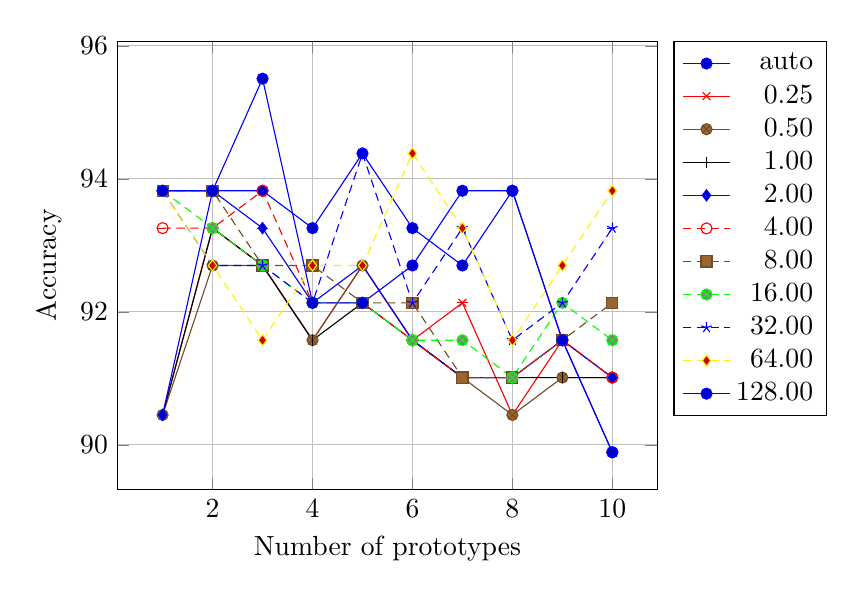
\begin{tikzpicture}
		\begin{axis}
		[
			yticklabel style={/pgf/number format/fixed,/pgf/number format/precision=3},
			ylabel={Accuracy},
			xlabel={Number of prototypes},
			grid=major,
			%height=7cm,
			%width=7cm,
			legend style={
				cells={anchor=east},
				%legend pos=south east,
				legend pos=outer north east,
			}
		]
		\addplot+[mark=*,error bars/.cd,y dir=both,y explicit]
		coordinates {
			(1,93.8202) +- (0,0)
			(2,93.8202) +- (0,0)
			(3,93.8202) +- (0,0)
			(4,93.2584) +- (0,0)
			(5,94.382) +- (0,0)
			(6,93.2584) +- (0,0)
			(7,92.6966) +- (0,0)
			(8,93.8202) +- (0,0)
			(9,91.573) +- (0,0)
			(10,89.8878) +- (0,0.0002)
		};
		\addlegendentry{auto}

		\addplot+[mark=x,error bars/.cd,y dir=both,y explicit]
		coordinates {
			(1,90.4494) +- (0,0)
			(2,93.2584) +- (0,0)
			(3,92.6966) +- (0,0)
			(4,91.573) +- (0,0)
			(5,92.6966) +- (0,0)
			(6,91.573) +- (0,0)
			(7,92.1348) +- (0,0)
			(8,90.4494) +- (0,0)
			(9,91.573) +- (0,0)
			(10,91.0112) +- (0,0)
		};
		\addlegendentry{0.25}	

		\/*
		\addplot+[error bars/.cd,y dir=both,y explicit]
		coordinates {
			(1,90.4494) +- (0,0)
			(2,92.6966) +- (0,0)
			(3,92.6966) +- (0,0)
			(4,91.573) +- (0,0)
			(5,92.6966) +- (0,0)
			(6,91.573) +- (0,0)
			(7,91.0112) +- (0,0)
			(8,90.4494) +- (0,0)
			(9,91.0112) +- (0,0)
			(10,91.0112) +- (0,0)
		};
		\addlegendentry{0.50}
		*/

		\addplot+[mark=|,error bars/.cd,y dir=both,y explicit]
		coordinates {
			(1,90.4494) +- (0,0)
			(2,93.2584) +- (0,0)
			(3,92.6966) +- (0,0)
			(4,91.573) +- (0,0)
			(5,92.1348) +- (0,0)
			(6,91.573) +- (0,0)
			(7,91.0112) +- (0,0)
			(8,91.0112) +- (0,0)
			(9,91.0112) +- (0,0)
			(10,91.0112) +- (0,0)
		};
		\addlegendentry{1.00}

		\/*
		\addplot+[error bars/.cd,y dir=both,y explicit]
		coordinates {
			(1,90.4494) +- (0,0)
			(2,93.8202) +- (0,0)
			(3,93.2584) +- (0,0)
			(4,92.1348) +- (0,0)
			(5,92.6966) +- (0,0)
			(6,91.573) +- (0,0)
			(7,91.0112) +- (0,0)
			(8,91.0112) +- (0,0)
			(9,91.573) +- (0,0)
			(10,91.0112) +- (0,0)
		};
		\addlegendentry{2.00}
		*/

		\addplot+[mark=o,error bars/.cd,y dir=both,y explicit]
		coordinates {
			(1,93.2584) +- (0,0)
			(2,93.2584) +- (0,0)
			(3,93.8202) +- (0,0)
			(4,92.1348) +- (0,0)
			(5,92.1348) +- (0,0)
			(6,91.573) +- (0,0)
			(7,91.0112) +- (0,0)
			(8,91.0112) +- (0,0)
			(9,91.573) +- (0,0)
			(10,91.0112) +- (0,0)
		};
		\addlegendentry{4.00}

		\/*
		\addplot+[error bars/.cd,y dir=both,y explicit]
		coordinates {
			(1,93.8202) +- (0,0)
			(2,93.8202) +- (0,0)
			(3,92.6966) +- (0,0)
			(4,92.6966) +- (0,0)
			(5,92.1348) +- (0,0)
			(6,92.1348) +- (0,0)
			(7,91.0112) +- (0,0)
			(8,91.0112) +- (0,0)
			(9,91.573) +- (0,0)
			(10,92.1348) +- (0,0)
		};
		\addlegendentry{8.00}
		*/

		\addplot+[color=green,error bars/.cd,y dir=both,y explicit]
		coordinates {
			(1,93.8202) +- (0,0)
			(2,93.2584) +- (0,0)
			(3,92.6966) +- (0,0)
			(4,92.1348) +- (0,0)
			(5,92.1348) +- (0,0)
			(6,91.573) +- (0,0)
			(7,91.573) +- (0,0)
			(8,91.0112) +- (0,0)
			(9,92.1348) +- (0,0)
			(10,91.573) +- (0,0)
		};
		\addlegendentry{16.00}

		\/*
		\addplot+[error bars/.cd,y dir=both,y explicit]
		coordinates {
			(1,93.8202) +- (0,0)
			(2,92.6966) +- (0,0)
			(3,92.6966) +- (0,0)
			(4,92.1348) +- (0,0)
			(5,94.382) +- (0,0)
			(6,92.1348) +- (0,0)
			(7,93.2584) +- (0,0)
			(8,91.573) +- (0,0)
			(9,92.1348) +- (0,0)
			(10,93.2584) +- (0,0)
		};
		\addlegendentry{32.00}
		*/

		\addplot+[color=yellow,error bars/.cd,y dir=both,y explicit]
		coordinates {
			(1,93.8202) +- (0,0)
			(2,92.6966) +- (0,0)
			(3,91.573) +- (0,0)
			(4,92.6966) +- (0,0)
			(5,92.6966) +- (0,0)
			(6,94.382) +- (0,0)
			(7,93.2584) +- (0,0)
			(8,91.573) +- (0,0)
			(9,92.6966) +- (0,0)
			(10,93.8202) +- (0,0)
		};
		\addlegendentry{64.00}

		\/*
		\addplot+[error bars/.cd,y dir=both,y explicit]
		coordinates {
			(1,93.8202) +- (0,0)
			(2,93.8202) +- (0,0)
			(3,95.5056) +- (0,0)
			(4,92.1348) +- (0,0)
			(5,92.1348) +- (0,0)
			(6,92.6966) +- (0,0)
			(7,93.8202) +- (0,0)
			(8,93.8202) +- (0,0)
			(9,91.573) +- (0,0)
			(10,89.8876) +- (0,0)
		};
		\addlegendentry{128.00}
		*/

		\end{axis}
	\end{tikzpicture}
\end{figure}
\end{frame}

\subsection{Iris Data Set}

\begin{frame}{Analysis of Self Training}
\begin{figure}
  \centering
	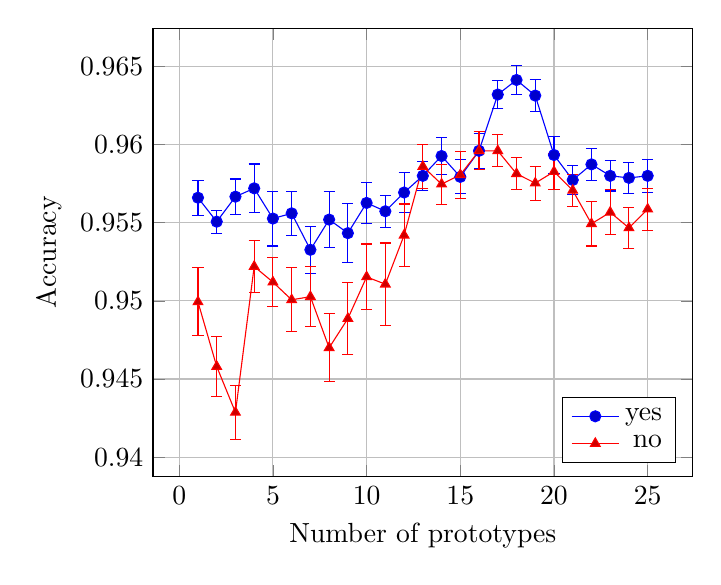
\begin{tikzpicture}
		\begin{axis}
		[
			yticklabel style={/pgf/number format/fixed,/pgf/number format/precision=3},
			ylabel={Accuracy},
			xlabel={Number of prototypes},
			grid=major,
			%height=7cm,
			%width=7cm,
			legend style={
				cells={anchor=east},
				legend pos=south east,
			}
		]
		% first
		\addplot+[error bars/.cd,y dir=both,y explicit]
		coordinates {
			(1,0.956600) +- (0.000000,0.001116)
			(2,0.955067) +- (0.000000,0.000730)
			(3,0.956667) +- (0.000000,0.001132)
			(4,0.957200) +- (0.000000,0.001559)
			(5,0.955267) +- (0.000000,0.001756)
			(6,0.955600) +- (0.000000,0.001398)
			(7,0.953267) +- (0.000000,0.001518)
			(8,0.955200) +- (0.000000,0.001802)
			(9,0.954333) +- (0.000000,0.001906)
			(10,0.956267) +- (0.000000,0.001298)
			(11,0.955733) +- (0.000000,0.001037)
			(12,0.956933) +- (0.000000,0.001299)
			(13,0.958000) +- (0.000000,0.000915)
			(14,0.959267) +- (0.000000,0.001196)
			(15,0.957933) +- (0.000000,0.001088)
			(16,0.959600) +- (0.000000,0.001106)
			(17,0.963200) +- (0.000000,0.000914)
			(18,0.964133) +- (0.000000,0.000920)
			(19,0.963133) +- (0.000000,0.001036)
			(20,0.959333) +- (0.000000,0.001190)
			(21,0.957733) +- (0.000000,0.000946)
			(22,0.958733) +- (0.000000,0.001040)
			(23,0.958000) +- (0.000000,0.000969)
			(24,0.957867) +- (0.000000,0.001010)
			(25,0.958000) +- (0.000000,0.001070)
	 	  %(26,95.8) +- (0,0.10695)
			%(27,95.7667) +- (0,0.08341)
			%(28,95.9067) +- (0,0.101245)
			%(29,95.9133) +- (0,0.1072)
			%(30,95.9133) +- (0,0.124855)
		};
		\addlegendentry{yes}
		%second
		\addplot+[mark=triangle*,error bars/.cd,y dir=both,y explicit]
		coordinates {
			(1,0.949933) +- (0.000000,0.002175)
			(2,0.945800) +- (0.000000,0.001926)
			(3,0.942867) +- (0.000000,0.001716)
			(4,0.952200) +- (0.000000,0.001664)
			(5,0.951200) +- (0.000000,0.001567)
			(6,0.950067) +- (0.000000,0.002045)
			(7,0.950267) +- (0.000000,0.001933)
			(8,0.947000) +- (0.000000,0.002182)
			(9,0.948867) +- (0.000000,0.002308)
			(10,0.951533) +- (0.000000,0.002106)
			(11,0.951067) +- (0.000000,0.002634)
			(12,0.954200) +- (0.000000,0.001996)
			(13,0.958600) +- (0.000000,0.001399)
			(14,0.957467) +- (0.000000,0.001277)
			(15,0.958067) +- (0.000000,0.001493)
			(16,0.959600) +- (0.000000,0.001223)
			(17,0.959600) +- (0.000000,0.001026)
			(18,0.958133) +- (0.000000,0.001030)
			(19,0.957533) +- (0.000000,0.001088)
			(20,0.958267) +- (0.000000,0.001133)
			(21,0.957067) +- (0.000000,0.001034)
			(22,0.954933) +- (0.000000,0.001421)
			(23,0.955667) +- (0.000000,0.001448)
			(24,0.954667) +- (0.000000,0.001307)
			(25,0.955867) +- (0.000000,0.001342)
			%(26,95.48) +- (0,0.17095)
			%(27,95.38) +- (0,0.15707)
			%(28,95.4667) +- (0,0.16215)
			%(29,95.4867) +- (0,0.180915)
			%(30,95.4133) +- (0,0.166595)
		};
		\addlegendentry{no}
    \end{axis}
	\end{tikzpicture}
\end{figure}
\end{frame}

\subsection{Flower Data Set}

\begin{frame}{Description}
	\begin{itemize}
		\item{1360 images from 17 species of some commom flowers in UK}
		\item{Very challenging dataset}
		\begin{itemize}
			\item{Large scale}
			\item{Viewpoints and light variations}
			\item{Classes with large variation of images within the class and close similarity to other classes}
		\end{itemize}
		\item{Flower vocabulary based on the petals of each flower}
			\begin{itemize}
				\item{Shape}
				\item{Colour}
				\item{Texture pattern}
			\end{itemize}
		% crucial information about the species
	\end{itemize}
\end{frame}

\begin{frame}{SS-CLAMP x SS-CARD}
\begin{figure}
	\centering
	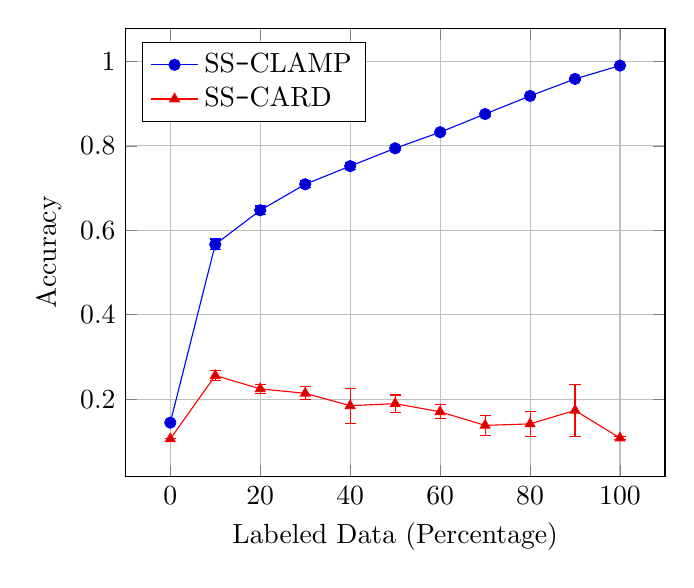
\begin{tikzpicture}
		\begin{axis}
		[
			ylabel=Accuracy,
			xlabel=Labeled Data (Percentage),
			grid=major,
			legend style={
				cells={anchor=west},
				legend pos=north west,
			}
		]
		\addplot+[error bars/.cd,y dir=both,y explicit]
		coordinates {
			(0,0.144412) +- (0.000000,0.004986)
			(10,0.566471) +- (0.000000,0.012990)
			(20,0.647353) +- (0.000000,0.010089)
			(30,0.708971) +- (0.000000,0.008338)
			(40,0.751912) +- (0.000000,0.007973)
			(50,0.794118) +- (0.000000,0.004295)
			(60,0.832206) +- (0.000000,0.006241)
			(70,0.875294) +- (0.000000,0.004885)
			(80,0.918088) +- (0.000000,0.002928)
			(90,0.958382) +- (0.000000,0.003199)
			(100,0.990000) +- (0.000000,0.000000)
		};
		\addlegendentry{SS\texttt{-}CLAMP}
		\addplot+[mark=triangle*,error bars/.cd,y dir=both,y explicit]
		coordinates {
			(0,0.105882) +- (0.000000,0.000000)
			(10,0.255882) +- (0.000000,0.011377)
			(20,0.224559) +- (0.000000,0.010835)
			(30,0.213824) +- (0.000000,0.015237)
			(40,0.184559) +- (0.000000,0.041137)
			(50,0.189412) +- (0.000000,0.020566)
			(60,0.170147) +- (0.000000,0.016328)
			(70,0.137941) +- (0.000000,0.023854)
			(80,0.141471) +- (0.000000,0.030146)
			(90,0.173382) +- (0.000000,0.062059)
			(100,0.108088) +- (0.000000,0.002794)
		};
		\addlegendentry{SS\texttt{-}CARD}
		\end{axis}
	\end{tikzpicture}
\end{figure}
\end{frame}

\begin{frame}{Prototypes obtained}
\begin{figure}
\centering
\subfigure[Sunflower?]{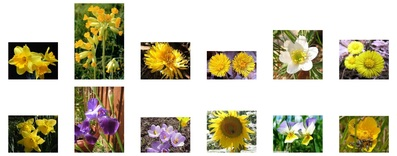
\includegraphics[width=0.74\textwidth]{image/F1.jpg}}
\subfigure[Sunflower ]{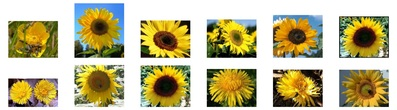
\includegraphics[width=0.74\textwidth]{image/F2.jpg}}
\end{figure}
\end{frame}

\begin{frame}{Prototypes obtained}
\begin{figure}
\centering
\subfigure[Windflower?]{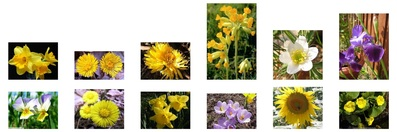
\includegraphics[width=0.74\textwidth]{image/F5.jpg}}
\subfigure[Windflower ]{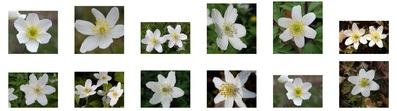
\includegraphics[width=0.74\textwidth]{image/F6.jpg}}
\end{figure}
\end{frame}

\section*{Summary}

\begin{frame}{Summary}
  \begin{itemize}
		\item{Semi-supervised algorithm to give a fuzzy partition and a set of prototypes for each cluster}
		\item{Intuitive approach to compute the $\alpha$}
		\item{Precision in calculating the new membership degree}
  \end{itemize}
  \vskip0pt plus.5fill
  \begin{itemize}
  \item{Outlook}
    \begin{itemize}
			\item{Extend this model to be simpler}
			\item{Investigate the possibility of improve the running time for compute the new prototypes}
    \end{itemize}
  \end{itemize}
\end{frame}

% references
\appendix
\section<presentation>*{\appendixname}
\subsection<presentation>*{For Further Reading}

\begin{frame}[allowframebreaks]
  \frametitle<presentation>{For Further Reading}
    
  \begin{thebibliography}{10}
    
  \beamertemplatebookbibitems
	
	\bibitem{chapele}
	O.~Chapelle, B.~Sch{\"o}lkopf, and A.~Zien, editors.
	\newblock {\em Semi-Supervised Learning}.
	\newblock MIT Press, Cambridge, MA, 2006.
    
  \beamertemplatearticlebibitems
	
	\bibitem{Frigui2008}
	H.~Frigui and Cheul Hwang.
	\newblock Fuzzy clustering and aggregation of relational data with instance-level constraints.
	\newblock {\em Trans. Fuz Sys.}, 16(6):1565--1581, December 2008.

  \end{thebibliography}
\end{frame}

% end
\end{document}
